\documentclass[acmsmall,screen,nonacm]{acmart}
\usepackage[T1]{fontenc}
\usepackage{microtype,float,graphicx,booktabs,tabularx,array,ragged2e,tikz,needspace,colortbl,placeins,longtable}
\usetikzlibrary{arrows.meta,positioning,calc}
\settopmatter{printacmref=false,printfolios=true,printccs=true}
\setcopyright{none}
\hypersetup{colorlinks=true,linkcolor=blue!50!black,citecolor=blue!50!black,urlcolor=blue!50!black}
\setlength{\emergencystretch}{2em}
\renewcommand{\topfraction}{.9}\renewcommand{\bottomfraction}{.9}\renewcommand{\textfraction}{.1}
\definecolor{unitshade}{HTML}{ECEFF3}
\providecommand{\doi}[1]{\href{https://doi.org/#1}{doi:#1}}
\newcolumntype{Y}{>{\RaggedRight\arraybackslash}X}
\newcolumntype{L}[1]{>{\RaggedRight\arraybackslash}p{#1}}
\title[Between the Issue and the Warning]{Between the Issue and the Warning\texorpdfstring{\\[0.25em]}{ }Issue Requirements and Security Warnings in Agent-Associated Pull Requests}
\hypersetup{pdftitle={Between the Issue and the Warning - Issue Requirements and Security Warnings in Agent-Associated Pull Requests}}
\author{Arno Strauss}
\affiliation{\institution{School of Computer Science and Applied Mathematics, University of the Witwatersrand}\city{Johannesburg}\country{South Africa}}
\email{2613224@students.wits.ac.za}
\renewcommand{\shortauthors}{Arno Strauss}
\begin{abstract}
Coding agents increasingly implement GitHub issues as pull requests (PRs), but a security-scanner finding alone does not show which PR change introduced the reported condition or how that change relates to the request. I examine 3,809 merged, issue-linked, agent-associated JavaScript/\allowbreak TypeScript instances, including 192 with recorded newly introduced findings. Detailed cases show issues requesting useful functionality that PRs implemented through security-relevant mechanisms the issues did not specify, including biased random-character selection, regex-based text repair and a check-then-read file sequence. An exploratory comparison of 190 matched pairs found less explicit implementation guidance in issues linked to finding-positive PRs than in their controls. In 12 complete retrospective replays, warning-informed inputs coincided with fewer recorded CodeQL alerts, but a single retained output per condition and unverified functionality prevent causal conclusions. The study links reported findings to specific changes without inferring hidden agent instructions or confirmed vulnerabilities.
\end{abstract}
\ccsdesc[500]{Software and its engineering~Software creation and management}
\ccsdesc[300]{Security and privacy~Software and application security}
\keywords{Empirical software engineering, coding agents, GitHub issues, security analysis, pull requests, implementation provenance}
\newlength{\crowW}
\newenvironment{casefile}[2]{\par\Needspace{9\baselineskip}\begingroup\fontsize{8}{9}\selectfont\renewcommand{\arraystretch}{1.18}\setlength{\crowW}{\dimexpr\linewidth-2.15cm-2\tabcolsep\relax}\noindent\begin{tabular}{@{}>{\bfseries\raggedright\arraybackslash}p{2.15cm}>{\raggedright\arraybackslash}p{\crowW}@{}}\toprule\rowcolor{unitshade}\multicolumn{2}{@{}>{\RaggedRight\arraybackslash}p{\linewidth}@{}}{\normalsize #1\par\smallskip\scriptsize #2}\\\midrule}{\bottomrule\end{tabular}\endgroup\par\medskip}
\newcommand{\crow}[2]{#1 & #2\\}
\begin{document}
\maketitle
\noindent\textit{2026 BSc Honours research paper. Supervisors: Prof. Michael Pradel (CISPA) and Prof. Hima Vadapalli (Wits).}

\section{Introduction}

Natural language has become an interface to software tools: a plain-text request can now be turned into code changes by a coding agent. On GitHub, an issue is usually a message to a maintainer, in which a user describes a defect or a wanted feature and a person decides how to implement it. Repository-capable coding agents now read the same text as a task, search the repository, edit code and open pull requests (PRs) \cite{b9,b20,b22,b25}, and such PRs appear in large numbers in open-source projects \cite{b11,b21}. Security analysis runs on this work as well: in a dataset of PRs that public signals attribute to coding agents, GitHub's rule-based security bot is among the ten most frequent bot reviewers \cite{b11}. Public issue intake has thereby become an input channel to automated code change.

That channel has a known weakness. Controlled studies show that crafted issue text can steer repair agents toward insecure or vulnerable patches that still pass tests, and that static analysis can miss them \cite{b3,b16}; prompt-injection benchmarks show that tool output and retrieved content can hijack agents, including coding editors \cite{b6,b12,b24}. These studies construct the attack, so they know which operation is responsible and what the issue was meant to cause. Naturally occurring work offers no such ground truth. A public issue--PR link is a starting point, not a record of every instruction or source the implementer saw, and links take several forms, including issues opened after the PR they are linked to \cite{b5}.

What the public record does expose is the outcome: security scanners report findings on agent-associated PRs. How does a reported finding relate to the work requested in the linked issue? It might concern code directly implementing the request, accompanying tests, or dependency changes produced by tooling. Issue-resolution benchmarks primarily measure task success \cite{b9}, while studies of coding-agent PRs describe their adoption and development patterns \cite{b11,b21}. Controlled security studies show that a patch can pass functional checks while introducing a weakness \cite{b3,b35}. This study connects scanner findings to the specific PR changes associated with them and to the requirements in the linked issue.

A concrete case shows why it matters. An \href{https://github.com/ZHANGTIANYAO1/teamspeak-music-bot/issues/112}{issue} in the teamspeak-music-bot project asks for Spotify as an audio source. The linked \href{https://github.com/ZHANGTIANYAO1/teamspeak-music-bot/pull/118}{pull request} delivers it, and in doing so builds a login verifier by turning each random byte into a character with a remainder operation over a 66-character alphabet. Because 256 byte values do not divide evenly into 66, some characters come up slightly more often than others, and CodeQL reports a biased-random warning. CodeQL identifies the flagged location, but the report alone does not establish which PR change introduced the condition or how that change relates to the request. The issue asked for Spotify support, not for this way of choosing characters.

I examine this gap in 3,809 merged, issue-linked, agent-associated JavaScript/\allowbreak TypeScript instances, including 192 with newly introduced scanner findings. The analysis uses public issue discussions, PR changes and tool output; these records reveal an implementation without establishing which instructions or context its author saw.

The central distinction is between addressing a task and assessing its security. A change can directly implement functionality described in an issue while also triggering a security warning. Interpreting that warning requires examining the changed code, its role in the task, and whether it affects production code, tests or documentation. The study examines these relationships rather than treating warning totals as a direct measure of security.


\subsection{Research Questions}\label{sec:rqs}

RQ1 examines how security findings relate to the requested work. RQ2 examines whether general implementation guidance differs between issues with and without new findings. RQ3 explores the code and scanner results produced when historical tasks receive additional security information. RQ1 provides the main evidence; the other analyses examine related questions about guidance.
\begin{itemize}
\item \textbf{RQ1.} How do security warnings in agent-associated pull requests relate to what their linked issues request?
\item \textbf{RQ2.} Does implementation guidance differ between issues linked to PRs with newly introduced findings and issues linked to matched PRs without new findings under comparable completed checks?
\item \textbf{RQ3.} In exploratory replays of historical tasks, how do the implementation and CodeQL findings differ when an issue is presented alone, with the historical warning, or with alternative forms of warning-derived safety guidance?
\end{itemize}

\subsection{Contributions}

The study shows that changes directly addressing a requested feature can also trigger security warnings, including warnings associated with implementation details the issue did not specify. It also shows why these warnings require interpretation: reports may concern tests or documentation, and several reports may arise from one underlying change. The matched comparison and exploratory replays examine issue specificity and additional security guidance without establishing their causal effects. The underlying mapping and classification methods are detailed in Sections~\ref{sec:attrib} and~\ref{sec:roles}.

\section{Background}

\subsection{Tasks, Patches and Coding Agents}

GitHub issues record requested functionality, defects and discussion; PRs record proposed changes. Their links permit analysing a request alongside a patch, but do not prove that the public issue initiated, fully specified or dictated the implementation \cite{b5}. Coding agents may also use repository instructions, files and tool output absent from the public issue \cite{b20,b22}. \emph{Agent-associated} means that public PR metadata, branch patterns or issue/PR text indicate coding-agent involvement; a tool mention does not prove agent authorship, so the sample is not a census of autonomously written patches.

\subsection{Warnings, Advisories and Retained Findings}

CodeQL and Semgrep flag patterns in source code; OSV and Trivy report vulnerable dependencies, while Gitleaks identifies possible secrets. CodeQL's query-based approach builds on QL, a language designed for querying program representations \cite{b44}. Throughout the paper, a \emph{finding} is one retained report from any of these tools, not a confirmed vulnerability. For RQ3, the recorded count is specifically the number of new CodeQL alerts in a generated patch.

A PR is \emph{finding-positive} when the recorded before/after comparison detects at least one new finding. A \emph{control} has no new findings under the applicable checks that completed successfully. Controls may still have older findings or lack results from other tools; neither label establishes exploitability or functional correctness.

\subsection{Task Relevance and Mechanism Choice}

\emph{Task role} describes how a change relates to the requested behaviour. Whether the issue specified the technique used is assessed separately.

\section{Related Work}

\subsection{Coding Agents and How They Are Judged}

SWE-bench evaluates software-repair patches against tests for 2,294 GitHub issues drawn from 12 Python repositories \cite{b9}. SWE-agent, AutoCodeRover and OpenHands provide repository-level interfaces for agents to inspect files, edit code and run tests \cite{b22,b25,b20}. Trae Agent studies test-time scaling for repository-level issue resolution by generating and selecting candidate solutions \cite{b47}. These systems and benchmarks primarily evaluate task completion; the present study instead examines the relationship between recorded security findings, the changes that produced them and the issue requirements.

\subsection{Agent Pull Requests and Issue Mining}

Public signals such as account identities, branch names and co-authorship metadata have been used to study coding-agent PRs at scale. Li et al. analyse agent participation in open-source development, while Watanabe et al. examine how agent-associated PRs are used and integrated on GitHub \cite{b11,b21}. The links between issues and PRs have their own structure and do not necessarily establish which public text initiated a change \cite{b5}. Prior issue research examines the requests made in open-source AI projects and the characteristics of beginner-friendly issues \cite{b23,b26}. This study uses issue links and coding-agent indicators to select its cohort, then inspects the code behind recorded findings rather than treating a link as proof of the instructions received by an agent.

\subsection{Crafted Issues and Untrusted Context}

Przymus et al. show that adversarial bug reports can lead automated repair agents to introduce attacker-aligned changes \cite{b16}. SWExploit constructs misleading issue reports intended to induce functionally correct but vulnerable patches \cite{b3}. AgentDojo and InjecAgent benchmark prompt injection through untrusted tool outputs and other external content; Liu et al. examine attacks against coding editors \cite{b6,b24,b12}. Related defenses study detecting and removing injected instructions (PromptArmor) and applying program analysis to agent runtime traces (AgentArmor) \cite{b45,b46}. These experiments investigate adversarial instructions or runtime defenses. This paper instead examines naturally occurring merged PRs without assuming that their linked issues are attacks.

\subsection{Static-Analysis Warnings and Generated Code}

Static-analysis findings need interpretation. Johnson et al. report that developers' use of static-analysis tools is affected by false positives and how the warnings fit their workflow \cite{b33}. Pearce et al. evaluate the security of code suggested by GitHub Copilot, showing why functional plausibility alone is not a security assessment \cite{b35}. The current study does not treat a scanner report as proof of exploitability; it identifies the changed operation associated with a report and examines whether that operation addresses an issue requirement or accompanies the work.

\subsection{Research Gap}

Benchmarks measure whether agents resolve tasks \cite{b9,b22}, mining studies characterise their PRs \cite{b11,b21}, and controlled attack studies investigate intentionally misleading inputs \cite{b3,b16}. This study examines how recorded scanner findings in merged, issue-linked agent-associated PRs relate to the concrete changes and requested behaviour. Its case analysis is the primary result; matched issue comparisons and retrospective replays examine related questions about guidance.

\section{Study Design and Methods}

I conduct an observational study of merged, agent-associated PRs linked to public GitHub issues in JavaScript and TypeScript repositories. The analysis follows the evidence from a requested task to the merged patch and the security findings recorded by static-analysis, dependency and secret-scanning tools. The study selects issue--PR instances and compares scanner results across each PR, links new findings to responsible changes (RQ1), compares issue wording with matched controls (RQ2), and examines a small set of retrospective warning-informed replays (RQ3). Figure~\ref{fig:overview} separates the observational comparisons from the replay study.

\Needspace{6\baselineskip}
One \emph{instance} is a linked issue--PR pair. A \emph{finding} is a retained scanner report; a \emph{responsible change} is the code or dependency operation linked to one or more findings. Related changes within an instance are grouped into an \emph{implementation choice}. The latter describes the selected technique, not a separate scanner finding. RQ2 analyses matched instance pairs; RQ3 analyses generated patches for selected historical tasks. Table~\ref{tab:population-guide} keeps their different populations separate.

\begin{table}[H]
\caption{Study populations and units. The subsets overlap and must not be added together.}
\label{tab:population-guide}
\footnotesize\renewcommand{\arraystretch}{1.10}
\begin{tabularx}{\linewidth}{@{}L{2.65cm}L{2.2cm}Y@{}}
\toprule
\textbf{Population} & \textbf{Size} & \textbf{Use in the paper}\\
\midrule
Full corpus & 3,809 instances & Merged, issue-linked PRs; scanner comparisons.\\
Finding-positive & 192 instances & At least one newly recorded finding.\\
Initial annotations & 122 instances & 605 findings linked to 322 responsible changes.\\
Extended mapped set & 191 instances & 455 responsible changes grouped into 342 implementation choices; one positive has no mapped change.\\
Matched comparison & 190 pairs & One positive and one control per RQ2 pair.\\
O/W/P replays & 14 tasks & 12 complete sets of three generated patches.\\
\bottomrule
\end{tabularx}
\end{table}

\begin{figure}[H]
\centering
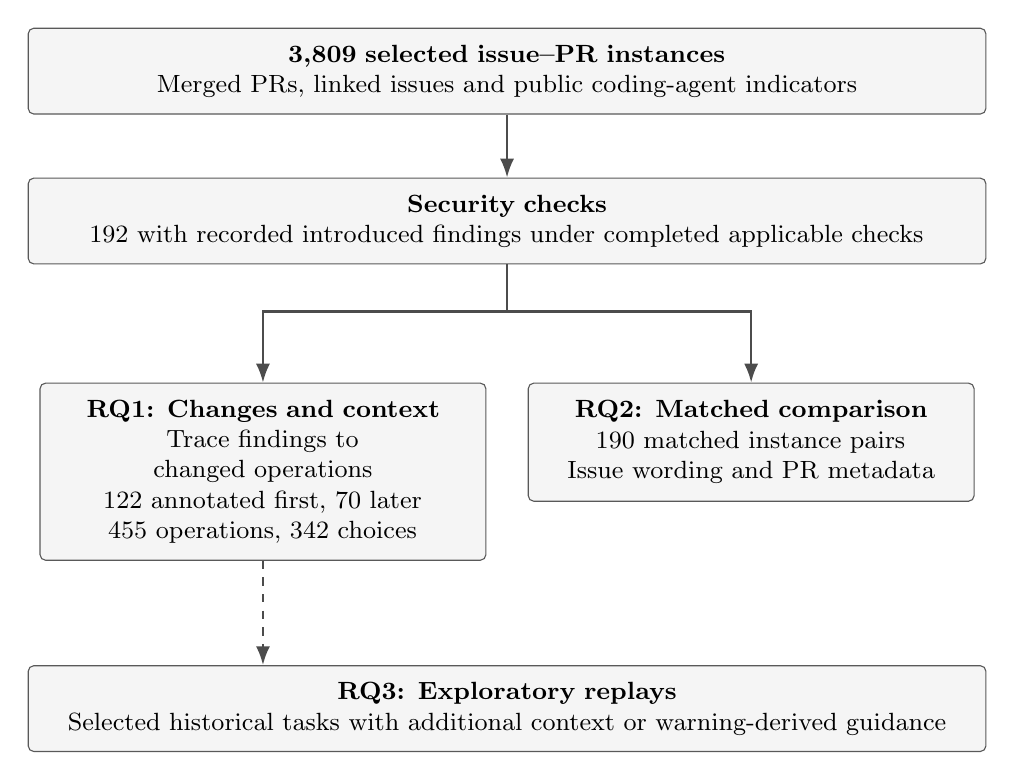
\begin{tikzpicture}[
  font=\small,>={Latex[length=2.4mm]},
  base/.style={draw=black!65,fill=black!4,rounded corners=2pt,align=center,inner xsep=8pt,inner ysep=6pt},
  wide/.style={base,text width=11.6cm},
  panel/.style={base,text width=5.1cm,minimum height=1.5cm},
  link/.style={->,line width=.9pt,draw=black!70},
  weak/.style={->,dashed,line width=.9pt,draw=black!70}]
  \node[wide] (cohort) {\textbf{3,809 selected issue--PR instances}\\ Merged PRs, linked issues and public coding-agent indicators};
  \node[wide,below=8mm of cohort] (checks) {\textbf{Security checks}\\ 192 with recorded introduced findings under completed applicable checks};
  \node[panel,anchor=north] (rq1) at ($(checks.south)+(-3.1cm,-1.5cm)$) {\textbf{RQ1: Changes and context}\\ Trace findings to changed operations\\ 122 annotated first, 70 later\\ 455 operations, 342 choices};
  \node[panel,anchor=north] (rq2) at ($(checks.south)+(3.1cm,-1.5cm)$) {\textbf{RQ2: Matched comparison}\\ 190 matched instance pairs\\ Issue wording and PR metadata};
  \node[wide,anchor=north] (rq3) at ($(rq1.south)!0.5!(rq2.south)+(0,-1.7cm)$) {\textbf{RQ3: Exploratory replays}\\ Selected historical tasks with additional context or warning-derived guidance};
  \draw[link] (cohort) -- (checks);
  \draw[line width=.9pt,draw=black!70] (checks.south) -- ++(0,-6mm) coordinate (fork);
  \draw[link] (fork) -| (rq1.north);
  \draw[link] (fork) -| (rq2.north);
  \draw[weak] (rq1.south) -- (rq1.south |- rq3.north);
\end{tikzpicture}
\caption{Study overview: the sampled population, the RQ1 attribution, the RQ2 matched comparison and the RQ3 replays. The dashed arrow shows that the replay tasks come from historical instances with CodeQL findings; RQ3 does not use the RQ2 pairs.}
\label{fig:overview}
\end{figure}

\subsection{Population and Selection}

Discovery searched GitHub for merged PRs linked to issues (qualifiers \texttt{is:pr}, \texttt{is:merged}, \texttt{linked:issue}) in non-archived JavaScript/\allowbreak TypeScript repositories with at least 100 stars, merged between 1 November 2025 and 11 August 2026. JavaScript and TypeScript match the CodeQL and Semgrep rule sets applied, the start date keeps the sample recent, and the star cutoff excludes very small repositories. The snapshot contains 3,809 distinct issue--PR instances in 723 repositories (609 JavaScript, 3,200 TypeScript; selection criteria and cohort characteristics in Table~\ref{tab:cohort}). Agent indicators include PR authorship or metadata, branch and description markers, and weaker issue-side references to Codex, Copilot, Cursor, Claude or Devin; for 236 instances the only association is an issue-side marker, not PR-side evidence. The 100-star threshold restricts the sample to more established repositories; it is a sampling filter rather than a quality measure. Stars and language are snapshot metadata, not values reconstructed at each merge date. The cohort is neither a random GitHub sample nor an estimate of finding prevalence among all coding-agent work.

\subsection{Detecting and Retaining Introduced Findings}

The pipeline records scanner applicability, execution and findings separately (Section~2.2). CodeQL and Semgrep findings are counted as introduced when the archived comparison reports them after, but not before, a PR. For the original cohort, retained source-code findings also have a primary or data-flow location on a PR-added line. These are \emph{introduced reports}, not independently established new vulnerabilities: a changed data-flow path may affect an existing flagged statement (Table~\ref{tab:scanners}).

Dependency results received an additional merge-base verification in the first annotation cohort. Package/version records were compared at the PR's true merge base and head; this verification excluded 12 initially positive instances after four earlier exclusions. Section~\ref{sec:s2} reports the checks and their results. Equivalent verification is not established for all 70 subsequently annotated positives, so I do not generalise the stronger verification claim to them.

Of the 3,809 instances, 192 had newly recorded findings. The remaining 3,617 had none under their completed applicable checks; this does not imply that every scanner ran. Detailed annotation covered 122 positives first and 70 later. One positive had no exactly mapped change, leaving the 191-instance mapped set in Table~\ref{tab:population-guide}. The original 122-instance batch was not a random sample. Its 605 findings and 322 responsible changes should not be confused with the 455 changes in the extended mapped set.

\subsection{Deduplication and Finding-to-Operation Attribution}\label{sec:attrib}

A finding and its responsible change are different: the scoped-package regex added in T3Code, for example, is associated with two distinct CodeQL rules that concern one regex-based strategy (Section~\ref{sec:s3}). Deduplication merged repeated records of a finding within an instance without merging distinct rules or advisories, yielding 605 findings from 832 raw tool references in the 122-instance cohort. For source-code warnings the comparison used reported rules and locations, changed hunks and available pre-change code; for dependency findings it used declared or resolved versions before and after the PR. A reported file location alone did not establish the responsible operation; Table~\ref{tab:mapping} gives the mapping basis of every finding.

I use model-assisted annotation to propose the code, configuration or dependency change responsible for each retained finding. The model received the scanner finding, tool evidence and PR diff, but not the issue text or PR description. A candidate link was retained only when the record identified a changed file, a line or diff hunk, and an explanation of how that change accounts for the finding. This records supporting evidence for each link, but does not constitute independent human verification of every link.

For 142 dependency findings in the original cohort, recorded merge-base verification supports the package/version attribution; 36 of these links were resolved during that verification. After exclusions, the 122-case workbook records 605 retained findings mapped to 322 changes (Table~\ref{tab:mapping}). The underlying dependency verification records and counts are given in Section~\ref{sec:s2}.

The recorded annotation model was GPT-5.6 Sol with medium reasoning effort. Because one responsible change can account for multiple findings, the two counts are reported separately. Independent validation limits are discussed in Section~\ref{sec:threats}. Subsequent task-role coding compares the mapped change with the issue's requested goals; it does not independently revalidate the finding-to-change link (Section~\ref{sec:roles}). Case evidence is presented in Sections~\ref{sec:s3} and~\ref{sec:s6}.

Figure~\ref{fig:rq1-method} shows how retained findings are linked to responsible changes, assigned task roles and grouped into implementation choices. Model-assisted grouping of the 455 changes yields 342 choices within instances. Each choice is classified as publicly prescribed, mechanically generated, selected among alternatives or unresolved, using only evidence available before the change (Table~\ref{tab:m1}). Choices made among alternatives are further described using the evidence tiers in Table~\ref{tab:rules-full}.

\begin{figure}[!tbp]
\centering
\includegraphics[width=0.9\textwidth]{figures/RQ1_Methodology.pdf}
\caption{Mapping findings to responsible changes and then to implementation choices. A blue bar at the left of a box marks a model-assisted step. Teal dashed callouts provide admissible evidence (the diff, issue or pre-introduction context); red marks an unsupported mapping or later evidence excluded from origin coding. Heavy dark outlines mark retained counts; the dashed final box denotes explanation tiers considered only for M choices. The yes/no arrows indicate whether a proposed link has supporting code evidence; they do not represent a statistical test. Retained links require a changed file, line or hunk and supporting explanation (Section~\ref{sec:attrib}).}
\label{fig:rq1-method}
\end{figure}

As a worked example, in Case~3 (Section~\ref{sec:rq1-open}) CodeQL's file-system-race report is the finding, the check-then-read sequence the PR added is the responsible change, and the read is Direct although the issue does not prescribe that sequence, so task role and implementation mechanism need separate annotations.

\subsection{Task Role, Artifact Context and Public Antecedents}\label{sec:roles}

Task role was coded per change by comparing a factual operation summary with the issue's requested goals (Table~\ref{tab:m1}). The labels (Direct, Supporting, Unclear) describe the operation's role, not whether its mechanism was publicly prescribed or who chose it. The annotations also record a finding family and an affected artifact: production source, tests or fixtures, documentation or examples, a dependency manifest, or a generated lockfile. The artifact category is recorded for the finding's reported location, such as a warning's primary location, which need not be the file that contains the mapped change. A pattern in a test or README does not imply the exposure of the same pattern in deployed code.

For the original 322 changes, an initial model-assisted pass assigned task roles using the frozen issue request and the change evidence, without PR-description text or complete finding records. A subsequent source-assisted quality-control pass revised 11 roles (seven Direct to Supporting and four Supporting to Direct); the workbook retains the earlier and final labels and case-specific reasons. These corrections do not constitute a second-annotator agreement study or independent revalidation of all links. The 133 later changes also have model-assisted roles.

The extended mapped set contains 455 responsible changes grouped into 342 implementation choices. Model-assisted coding then asks whether each technique was prescribed in public evidence before the change, followed mechanically from tools or dependency resolution, or was selected among plausible alternatives. Unresolved is allowed where evidence is insufficient (Table~\ref{tab:m1}). For choices made among alternatives, a separate classification describes the strength of any earlier public precedent. The primary counts use one retained classification version; the comparison with an earlier version is confined to Table~\ref{tab:routes}. Independent blind human agreement was not measured.

Public antecedents were judged against the recorded introduction chronology. A pre-existing helper or discussion is a possible source, not evidence that the contributor viewed it. Issue timestamps can postdate PR creation: in the original 122 instances, 4 PRs were opened before their linked issue and 15 more within 10 minutes after it. These are PR creation times, not the time the implementing code first appeared, and the public issue may omit private user or agent messages. A link between an issue and a PR thus does not show that the agent worked from that issue, and a Direct role records semantic alignment with the public issue's goals, not that the issue preceded, initiated or caused the change. Neither an absent antecedent nor a mechanism's first appearance in a patch therefore establishes autonomous invention.

\begin{table}[!tbp]
\caption{RQ1 decision rules and non-equivalences. Task role is decided per responsible change; the origin per grouped choice.}
\label{tab:m1}
\fontsize{8}{10}\selectfont\renewcommand{\arraystretch}{1.1}
\begin{tabularx}{\linewidth}{@{}L{2.5cm}YY@{}}
\toprule
\textbf{Category} & \textbf{Decision rule} & \textbf{Interpretation}\\
\midrule
\multicolumn{3}{@{}l}{\textit{Task role (per responsible change)}}\\
\textbf{Direct} & Implements a substantive goal of the public issue. & The issue need not prescribe the mechanism.\\
\textbf{Supporting} & Enables or accompanies the requested work rather than fulfilling it, including incidental implementation choices the issue did not request. & Role is not inferred from file type alone.\\
\textbf{Unclear} & Evidence cannot establish the task relation. & Uncertainty is retained, not forced into a binary.\\[2pt]
\multicolumn{3}{@{}l}{\textit{How the implementation choice arose (per grouped choice)}}\\
\textbf{H: prescribed} & Pre-introduction public evidence specifically fixes the mechanism. & A broad goal or later evidence is insufficient.\\
\textbf{T: mechanical} & Dependency resolution, generated artifacts or tooling produce the choice. & Not evidence of discretionary choice.\\
\textbf{M: selected among alternatives} & One implementable technique was used although public evidence did not require it and plausible alternatives exist. & A known precedent may explain the choice; its source is not established.\\
\textbf{U: unresolved} & Evidence cannot separate H, T and M. & Missing evidence is not proof of choice.\\
\midrule
\textbf{Earlier public evidence} & For M choices, note any reused code, repository precedent, stated contract or contextual support. & Its availability does not show that the contributor saw it.\\
\bottomrule
\end{tabularx}
\end{table}

\subsection{Matched Controls and Issue Coding}\label{sec:rq2-design}

RQ2 compares how issues are worded in finding-positive instances and in matched controls with no newly introduced finding under the checks that applied and completed. A control is not thereby secure: it may carry older findings, and not every tool ran on it. The recorded matching procedure paired each PR with new findings with at most one control PR without recorded new findings. Issue-wording annotations were joined after matching. Controls had to include the positive instance's completed applicable scanner checks, fall within 90 days of its PR creation date and stay within roughly fourfold of its changed-line and changed-file counts. The matcher preferred controls from the same repository. Issue wording, review variables and agent identity were not additional matching criteria (Figure~\ref{fig:rq2-method}; protocol in Section~\ref{sec:s5}). Of the 192 positives, 190 were matched (115 same-repository, 75 cross-repository; Table~\ref{tab:rq2-diag}). These are frozen matching records and not a rerun of the optimisation. Matching does not equate the tasks or randomise the wording.

Each issue received one of three wording labels: Problem only, Suggests solution or Explicit instruction. They describe the specificity of wording, not whether a security requirement was stated or the exact mechanism prescribed; Explicit instruction is not the choice-level H origin. Positive issues and controls were coded in separate passes; the control pass withheld scanner outcomes and pair identities. Because cross-pass agreement was not measured, some of the wording difference could reflect coding differences (Section~\ref{sec:threats}). The 121 original-cohort pairs and the 115 same-repository pairs are nested sensitivity subsets, not independent replications. The matched pair is the unit of analysis. I use a paired Stuart--Maxwell test to compare the three issue-wording categories. The primary test was recomputed from its frozen contingency table (Table~\ref{tab:rq2}); the Holm adjustment within a family of nine comparisons and the secondary comparisons are taken from the archived analysis (Section~\ref{sec:s5}). The comparison is observational; its other limitations are discussed in Section~\ref{sec:threats}.

\subsection{Retrospective and Information-Guided Replays}\label{sec:rq3-design}

The RQ3 replays are a retrospective diagnostic, separate from the RQ2 pairs (definitions and protocols in Section~\ref{sec:s6}). Fourteen historical tasks were assigned three input conditions: O, the original issue; W, the issue with its historical CodeQL warning; and P, the issue with a security property derived from that warning without naming the rule. W and P were constructed using historical warnings. The experiment therefore does not establish whether equivalent guidance could be identified before implementing a new task. Of 42 intended outputs, 40 are retained (12 O, 14 W and 14 P), giving 12 complete O/W/P triples; the two missing O outputs are not imputed. One archived output is available per retained task and condition. The records link these outputs to scan results and baseline identifiers, but do not establish comparable, independent model sessions or functional equivalence across conditions. The tasks were selected for prior CodeQL warnings rather than sampled randomly.

Additional pilots are documented in Section~\ref{sec:s6}; unresolved generation provenance prevents their use as evidence of an instruction effect.

New CodeQL alerts, including those sharing the historical rule, are reported for the 12 complete triples against their recorded baselines (Table~\ref{tab:replays}). The separate guidance pilot is described only in Section~\ref{sec:s6}.

\section{Results}

Warnings were not confined to changes unrelated to the requested task. In several examined cases, they concerned code directly addressing the request, while the issue left the flagged implementation detail unspecified. Other findings occurred in tests or documentation and did not by themselves establish exposure in deployed software. The results therefore distinguish a finding's relationship to the task from its implications for production use. The mapping and classification methods are described in Sections~\ref{sec:attrib} and~\ref{sec:roles}.

\subsection{RQ1: Findings Versus Changed Operations}\label{sec:rq1-roles}

In the first 122 finding-positive instances annotated, 605 scanner findings were linked to 322 responsible changes. A single change can generate several reports, so these totals represent different things. For example, the \href{https://github.com/Pimzino/spec-workflow-mcp/pull/173}{spec-workflow-mcp PR} refreshed a lockfile while addressing a path-translation problem; its 131 dependency-related findings mapped to 36 changes. Figure~\ref{fig:concentration} shows how a handful of instances dominate the warning totals. Detailed counts are in Table~\ref{tab:concentration}.

\begin{figure}[!tbp]
\centering
\includegraphics[width=0.7\linewidth]{figures/Fig5_Concentration.pdf}
\caption{A few instances hold many findings but almost none of the source-code changes. Each bar splits one total between the seven instances with the most findings and the other 115 in the original cohort. The seven hold 52\% of all findings but only 3\% of source-code responsible changes. Counts for the seven are the totals minus the excluded-seven counts in Table~\ref{tab:concentration}.}
\label{fig:concentration}
\end{figure}

Seven PRs account for more than half of the scanner reports but only five of the 166 mapped source-code changes. Much of this concentration reflects dependency findings and repeated data-flow reports. Finding totals therefore describe a different distribution from the underlying code changes; Figure~\ref{fig:concentration} and Table~\ref{tab:concentration} provide the detailed breakdown.

The relationship to the requested task also varies by finding family (Table~\ref{tab:role}). Task role is assigned to each responsible change, not inferred from the number of warnings it produced.

\begin{table}[!tbp]
\caption{Findings and responsible changes by finding family and task role.}
\label{tab:role}
\small
\begin{tabular}{@{}l>{\columncolor{unitshade}}r@{\hspace{10pt}}rrrr@{}}
\toprule
& \multicolumn{1}{>{\columncolor{unitshade}}c}{\textbf{Findings}} & \multicolumn{4}{c}{\textbf{Responsible changes (task role)}}\\
\cmidrule(l{2pt}r{2pt}){2-2}\cmidrule(l){3-6}
\textbf{Finding family} & \multicolumn{1}{>{\columncolor{unitshade}}r}{Reported} & \textbf{Total} & Direct & Supporting & Unclear\\
\midrule
Source-code warnings & 294 & \textbf{166} & 82 & 82 & 2\\
Dependency advisories and downgrades & 290 & \textbf{137} & 4 & 132 & 1\\
Secret-like findings & 18 & \textbf{16} & 3 & 13 & 0\\
Other dependency-version changes & 3 & \textbf{3} & 2 & 1 & 0\\
\midrule
Total & 605 & \textbf{322} & 91 & 228 & 3\\
\bottomrule
\end{tabular}
\par\smallskip\raggedright\footnotesize Original 122 finding-positive instances. A finding is one deduplicated tool report; a responsible change is the changed operation to which one or more findings were mapped, and task role is coded per responsible change. Not the extended 455-change population (Section~\ref{sec:s4}).
\end{table}

A scanner's reported location need not identify the responsible PR change. In the original cohort, data-flow reports often pointed outside the modified test code, sometimes producing many reports from a few changed operations. The detailed location-mapping and sensitivity counts are retained in Section~\ref{sec:s4}.

The affected file also matters. In Paperclip, file-system warnings arose in added regression tests; in dot-ai, a Gitleaks finding concerned a token placeholder in documentation. Neither finding alone establishes exposure in deployed code (source-linked records in Section~\ref{sec:s3}). The wider set contains CodeQL findings in both production code and tests (Figure~\ref{fig:scanner}).

\subsection{RQ1: Requested Behaviour Versus Implemented Mechanism}\label{sec:rq1-open}

A Direct role says that an operation implements what the issue asked for, not that the issue chose how. The three cases show distinct ways a requested feature can be implemented through a security-relevant technique that the issue did not specify. They are explanatory examples, not a prevalence sample. Each card identifies the request, the implemented operation, the resulting warning, an alternative approach and the limits of what public evidence can establish. Additional source-linked case evidence is provided in Section~\ref{sec:s3}.

\begin{casefile}{\textbf{Case 1: Spotify login verifier}\ \ {\scriptsize\texttt{ZHANGTIANYAO1/\allowbreak teamspeak-music-bot}}}{\href{https://github.com/ZHANGTIANYAO1/teamspeak-music-bot/issues/112}{Issue \#112}\ \ \href{https://github.com/ZHANGTIANYAO1/teamspeak-music-bot/pull/118}{PR \#118}}
\crow{Request}{Add Spotify as an audio source next to existing music services. The issue suggests a solution but says nothing about how the login verifier is built.}
\crow{What the PR did}{Builds the verifier by turning each random byte into a character with a remainder operation over a 66-character alphabet. 256 is not a multiple of 66, so some characters are slightly more likely.}
\crow{Warning}{CodeQL: biased random value in a cryptographic setting.}
\crow{Reading}{The change implements the requested Spotify service and is classified as Direct, but the issue did not prescribe how to generate the verifier. The character distribution is non-uniform; exploitability was not assessed. The case illustrates an implementation-level warning rather than a confirmed vulnerability.}
\crow{Alternative}{The pre-PR repository already used \texttt{randomBytes(32).toString("base64url")} for session tokens in \href{https://github.com/ZHANGTIANYAO1/teamspeak-music-bot/blob/f8743a904f50a065c9fcf5139e46005b5fff2e46/src/data/sessions.ts\#L56}{\texttt{src/data/sessions.ts:56}}. This is a local example of random-token encoding without modulo reduction, but it was not evaluated as a drop-in replacement for the Spotify verifier. RFC 7636 describes this encoding method for generating a PKCE verifier \cite{b39}.}
\crow{Open question}{Whether repository habit, an unseen prompt or the model\textquotesingle s default led here cannot be told from the public record.}
\end{casefile}

\begin{casefile}{\textbf{Case 2: GSD tool-call repair}\ \ {\scriptsize\texttt{gsd-build/\allowbreak gsd-2}}}{\href{https://github.com/gsd-build/gsd-2/issues/2660}{Issue \#2660}\ \ \href{https://github.com/gsd-build/gsd-2/pull/3090}{PR \#3090}}
\crow{Request}{Milestone completion fails when the model writes YAML-style bullet lists into JSON tool arguments. The issue suggests making the JSON format clearer in prompts, templates or schema hints.}
\crow{What the PR did}{For the final tool-call arguments, the PR attempts strict parsing, uses a regular expression to repair bullet lists if that fails, and can fall back to a streaming parser. Other streaming paths are not assumed to follow this exact sequence.}
\crow{Warning}{CodeQL: a regular expression that can take polynomial time on crafted input.}
\crow{Reading}{Direct, because the repair delivers the requested recovery. A regular-expression repair was not among the remedies the issue suggested.}
\crow{Alternative}{The remedies the issue itself named, or a repair that scans the text once without a backtracking pattern. The first is observed in the issue, the second is general practice.}
\crow{Open question}{Whether a maintainer steered the agent toward runtime repair, or the agent preferred it, cannot be told.}
\end{casefile}

\begin{casefile}{\textbf{Case 3: Grok CLI file mentions}\ \ {\scriptsize\texttt{superagent-ai/\allowbreak grok-cli}}}{\href{https://github.com/superagent-ai/grok-cli/issues/235}{Issue \#235}\ \ \href{https://github.com/superagent-ai/grok-cli/pull/236}{PR \#236}}
\crow{Request}{Load files referenced with @-mentions into the prompt (Explicit instruction).}
\crow{What the PR did}{Looks up the path\textquotesingle s metadata and checks it is not a directory, then reads the file in a separate step. The file can change in between.}
\crow{Warning}{CodeQL: file-system race (check, then use).}
\crow{Reading}{Direct. The issue did not prescribe a check-then-read sequence.}
\crow{Alternative}{Open the file once and read through that handle. A replay on a different file-access task generated a similar pattern (Section~\ref{sec:rq3-res}); this does not establish what the Grok CLI implementer considered.}
\crow{Open question}{The public record shows no instruction for it. Whether anything unseen did cannot be told.}
\end{casefile}

These cases illustrate the distinction; they do not estimate its frequency across agent development.

\begin{table}[H]
\caption{Selected cases illustrating the difference between task relevance and the warning-producing detail. These examples are not a prevalence sample.}
\label{tab:case-synthesis}
\footnotesize\renewcommand{\arraystretch}{1.14}
\begin{tabularx}{\linewidth}{@{}L{1.85cm}L{1.55cm}L{3.05cm}Y@{}}
\toprule
\textbf{Case} & \textbf{Task role} & \textbf{Flagged detail} & \textbf{What the case establishes}\\
\midrule
Spotify & Direct & Modulo-based verifier generation & The request did not prescribe this token-generation method.\\
GSD tool-call repair & Direct & Regex-based repair of malformed arguments & Runtime repair was implemented instead of the prompt or schema remedies proposed in the issue.\\
Grok file mentions & Direct & Separate metadata check and pathname read & The requested file loading did not prescribe this access sequence.\\
Paperclip & Supporting test code & File checks and reads in regression tests & A PR warning does not by itself establish production exposure.\\
\bottomrule
\end{tabularx}
\end{table}

The cases illustrate different mechanisms rather than a single generic failure. Spotify uses a biased character-mapping step in an authentication flow; GSD implements runtime text repair instead of the prompt or schema guidance suggested in its issue; and Grok CLI introduces a file check that creates a check-then-use race. In all three, the issue requests the behaviour without specifying the warning-producing operation. These observations locate the security-relevant distinction in the implementation, but do not establish why the implementer selected it. Four further cases (Neo.mjs, T3Code, KIRI, Paperclip; Section~\ref{sec:s3}) show related distinctions. The Chaibuilder case shows why task role and mechanism need separate labels. The issue requested Tailwind CSS v3, so changing its dependency constraint addresses the request. The six dependency entries associated with advisory reports were classified as Supporting; this does not establish that the downgrade necessarily produced each entry.

The full classification of 342 implementation choices and its version-sensitivity analysis are reported in Section~\ref{sec:s4}. These model-assisted counts are supporting evidence; the cases above illustrate the implementation mechanisms rather than the frequency of any one explanation.

\subsection{RQ2: Issue Specificity in Matched Instances}\label{sec:rq2-res}

Explicit implementation instructions were less common in issues linked to PRs with new findings than in matched controls: 63.7\% versus 77.9\%, a difference of 14.2 percentage points (95\% confidence interval approximately 5.6--22.8; Holm-adjusted $p=0.00468$). This measures general implementation specificity, not security guidance. Because the groups were coded in separate passes, coding differences may also contribute to the contrast. Table~\ref{tab:rq2} reports the paired categories; additional comparisons and sensitivity subsets are in Section~\ref{sec:s5}.

\begin{table}[H]
\caption{Issue wording in 190 matched pairs. Rows: finding-positive issues; columns: matched controls with no newly introduced findings under completed applicable checks.}
\label{tab:rq2}
\small
\begin{tabular}{@{}lrrrr@{}}
\toprule
& \multicolumn{3}{c}{\textbf{Control issue wording}} & \\
\cmidrule(lr){2-4}
\textbf{Positive issue} & Explicit instruction & Problem only & Suggests solution & Total\\
\midrule
Explicit instruction & 98 & 15 & 8 & 121\\
Problem only & 25 & 10 & 1 & 36\\
Suggests solution & 25 & 8 & 0 & 33\\
\midrule
Total & 148 & 33 & 9 & 190\\
\bottomrule
\end{tabular}
\par\smallskip\raggedright\footnotesize Positive labels were frozen in earlier annotation stages; control labels were produced later from blinded packets. Stuart--Maxwell $\chi^2(2)=15.12$, $p=0.00052$ ($p_{\mathrm{Holm}}=0.00468$). Matching diagnostics and subset results: Section~\ref{sec:s5}.
\end{table}

The GSD tool-call case (Case~2) illustrates the distinction. Its finding-positive \href{https://github.com/gsd-build/gsd-2/issues/2660}{issue} suggested prompt, template or schema remedies and was classified as suggesting a solution. Its same-repository control, \href{https://github.com/gsd-build/gsd-2/issues/2545}{issue \#2545}, specified expected operations and files for a queue command and was classified as an explicit instruction. The tasks differ, so this pair illustrates the coding categories rather than an effect of issue wording.

\subsection{RQ3: Alerts and Implementations in Replays}\label{sec:rq3-res}

\input{tables/owp_replays.tex}

Across the 12 tasks with all three conditions, recorded new CodeQL alerts totalled 21 for the issue alone, 10 with the historical warning and 15 with a warning-derived property (Table~\ref{tab:replays}). These are comparisons between separately generated patches. Warning-informed patches were often smaller, and functional equivalence was not established. The results therefore describe differences in scanner outcomes rather than demonstrated security improvement.

\begin{casefile}{\textbf{Case 4: cc-wf-studio replay}\ \ {\scriptsize\texttt{breaking-brake/\allowbreak cc-wf-studio}}}{\href{https://github.com/breaking-brake/cc-wf-studio/issues/683}{Issue \#683}\ \ \href{https://github.com/breaking-brake/cc-wf-studio/pull/695}{PR \#695}}
\crow{Request}{An independent commentary session that narrates workflow execution in a chat panel (Explicit instruction).}
\crow{Historical PR}{A watcher checks a log file\textquotesingle s size by pathname, then separately opens that path and reads through the resulting file descriptor. CodeQL reported a file-system race.}
\crow{Replay}{Original issue alone (O): the same two separate steps. With the warning added (W): one open file used for both size and reading. With a safety property added (P): the same, through a single handle.}
\crow{Reading}{The warning-informed generation used a single-handle access pattern instead of the separate size-check/read operations. One generation per arm cannot distinguish the effect of this information from run-to-run variation.}
\crow{Limit}{New alerts were 3, 1 and 1, with the historical rule only under O. A reconstructed rerun did not reproduce two archived rule hits, and functional equivalence was not checked.}
\end{casefile}

The cc-wf-studio outputs also differed in file-access behaviour: the warning-informed conditions used one open file for metadata inspection and reading. This provides a concrete example of different generated code under additional guidance, without establishing a causal effect.

\section{Discussion}

\subsection{Requested Behaviour and Unspecified Mechanisms}

Under a controlled attack, patches that pass the tests can carry injected vulnerabilities \cite{b3}. The cases here examine naturally occurring agent-associated PRs rather than constructed attacks. The linked issue states a goal, the PR implements a particular mechanism, and static analysis flags a pattern for which another implementation is available. The public record does not establish whether an attacker was involved, whether the chosen mechanism was functionally correct, or who selected it. Possible alternatives include standard URL-safe encoding for the Spotify verifier, the prompt or schema changes proposed in the GSD issue, and a single file handle instead of separate checks and reads in Grok CLI. At the pre-PR revision, the Spotify repository already used URL-safe encoding of random bytes for a separate session token. This is a local example, not evidence that the implementation author saw it or that it was a tested replacement for the verifier. A separate cc-wf-studio replay generated a single-handle pattern when given warning information. In these examples, the public issues did not specify the particular flagged operation.

Task role and mechanism prescription are distinct. Both the GSD runtime repair and the Grok CLI file read directly address their issues, but their warning-producing techniques were not specified in those issues. A security warning thus says little on its own about whether the changed operation served the task.

\subsection{What Could Explain a Mechanism Choice}\label{sec:explain}

The public records establish the implementation and sometimes show earlier repository precedent or an alternative described in the issue; they do not establish why the historical contributor used a particular technique. Possible explanations include following existing project helpers or generated code, instructions outside the linked issue, patterns learned by the model, and the issue's own suggested approach. A linked issue does not establish the instructions the agent received; some linked issues were created after the PR. The cc-wf-studio replay generated a single-handle file-access pattern under warning-informed input, providing an observed alternative without identifying the cause of the historical implementation.

\subsection{Remaining Validation and Future Comparisons}

RQ3 has already explored historical-warning feedback, warning-derived properties and alternative levels of implementation guidance. Those preliminary interventions produced different CodeQL counts and, in some cases, different mechanisms, but the available outputs do not establish independent effects or preserved task functionality. The next experiment should validate these effects rather than repeat the same preliminary design: record the complete model inputs and repository context, independently regenerate the unmodified issue several times, and retain cases where the historical mechanism or warning can be reproduced while the task is completed. On those cases, isolate one treatment at a time, compare sufficiently replicated issue-guidance and repository-precedent conditions, and apply the same historical rule to the unchanged pre-PR base and each generated patch. Functional tests and review of the exact responsible mechanism are needed alongside the scanner outcomes to determine whether the additional information actually prevents a warning-producing implementation. Comparing similarly selected PRs without agent markers would then test whether the observed patterns are specific to agent-associated work.

An additional experiment could test whether retrieving repository precedents and alternative implementations before code generation changes mechanism selection. Such a study would need to record agent context and compare generated patches under repeated runs; the present replays do not evaluate this retrieval strategy.

\section{Threats to Validity}\label{sec:threats}

\paragraph{Attribution and annotation.} Finding-to-change links and many task-role and mechanism-origin labels were proposed by a language model and retained under the stated evidence rules (Section~\ref{sec:attrib}). The original workbook documents 11 task-role corrections but does not establish complete, independent human review of the 605 links or a second-annotator agreement rate. These model-assisted annotations should not be treated as independent human ground truth. Findings about change roles, concentration and mechanism routes therefore inherit annotation uncertainty. Four of the 122 original PRs predate their linked issue, and 15 more were opened within ten minutes afterward. Together with uncertain agent association, this limits any claim about what instructions produced the code.

\paragraph{Sampling and measurement.} The corpus is selected using public agent markers, merge status, issue links, language and repository popularity, not verified line-by-line agent authorship. The original 122 positives form an initial annotation batch, not a random sample; no human-authored comparison is available. One dependency change can generate many advisory reports, which drives the concentration result. For 159 findings supported by changed data-flow locations, the archived before/after comparison cannot by itself exclude a previously existing flagged statement whose flow changed. A scanner warning is not a confirmed exploitable vulnerability, and a scan without new findings is not proof of secure code. Test fixtures, documentation and lockfiles also have different exposure implications from deployed source.

\paragraph{Matching and replay.} The paired wording statistic is reproducible from Table~\ref{tab:rq2}, but matching does not control task content or all confounders. Positive and control wording labels were produced in different annotation passes without a cross-pass agreement estimate. Stronger merge-base dependency verification is evidenced for the original annotation cohort only; the comparison therefore retains possible measurement differences. The observed wording difference is an association, not an effect. RQ3 uses retrospectively selected tasks, hindsight-derived inputs and one retained output per condition. Archived alert totals were not independently regenerated and generated patches were not functionally validated, so fewer alerts cannot establish prevention or repair.

\section{Conclusion}

The cases show why task relevance and security assessment must be considered separately. Security findings arose in changes directly related to requested behaviour, including implementation details that the issues left open. Other reports concerned accompanying tests, documentation or dependencies, where the meaning of a warning differs from one in production source.

The matched comparison found less explicit implementation guidance in issues linked to PRs with new findings, while the exploratory replays recorded different scanner outcomes and file-access patterns under additional warning-derived information. These secondary observations motivate more controlled investigation rather than establishing a preventive effect. Connecting findings to the changed code and the public request makes clear which security-relevant details the issue left unspecified and which reports concern accompanying tests or documentation.

\section*{Data and Code Availability}

The study data and code can be found in the \href{https://github.com/Stralb/adversarial-swe-agents}{project repository}.

\clearpage
\raggedbottom
\begingroup
\begin{thebibliography}{99}
\fontsize{8}{9}\selectfont
\setlength{\itemsep}{0pt}
\setlength{\parsep}{0pt}
\setlength{\parskip}{0pt}
\bibitem{b44} Pavel Avgustinov, Oege de Moor, Michael Peyton Jones, and Max Sch\"afer. 2016. QL: Object-oriented Queries on Relational Data. In \emph{30th European Conference on Object-Oriented Programming (ECOOP 2016)}, Leibniz International Proceedings in Informatics, Vol. 56. Schloss Dagstuhl--Leibniz-Zentrum f\"ur Informatik, Dagstuhl, Germany, Article 2, 2:1--2:26. \doi{10.4230/LIPIcs.ECOOP.2016.2}
\bibitem{b3} Simin Chen, Yixin He, Suman Jana, and Baishakhi Ray. 2025. Red Teaming Program Repair Agents: When Correct Patches can Hide Vulnerabilities. arXiv:2509.25894v1. \url{https://arxiv.org/abs/2509.25894v1}
\bibitem{b6} Edoardo Debenedetti, Jie Zhang, Mislav Balunovi\'c, Luca Beurer-Kellner, Marc Fischer, and Florian Tram\`er. 2024. AgentDojo: A Dynamic Environment to Evaluate Prompt Injection Attacks and Defenses for LLM Agents. In \emph{Advances in Neural Information Processing Systems}, Vol. 37. Curran Associates, Inc., 82895--82920. \doi{10.52202/079017-2636}
\bibitem{b5} Cleidson R. B. de Souza, Emilie Ma, Jesse Wong, Dongwook Yoon, and Ivan Beschastnikh. 2024. Revealing Software Development Work Patterns with PR-Issue Graph Topologies. \emph{Proceedings of the ACM on Software Engineering} 1, FSE, Article 106 (July 2024), 22 pages. \doi{10.1145/3660813}
\bibitem{b47} Pengfei Gao, Zhao Tian, Xiangxin Meng, Xinchen Wang, Ruida Hu, Yuanan Xiao, Yizhou Liu, Zhao Zhang, Junjie Chen, Cuiyun Gao, Yun Lin, Yingfei Xiong, Chao Peng, and Xia Liu. 2025. Trae Agent: An LLM-based Agent for Software Engineering with Test-time Scaling. arXiv:2507.23370. \doi{10.48550/arXiv.2507.23370}
\bibitem{b9} Carlos E. Jimenez, John Yang, Alexander Wettig, Shunyu Yao, Kexin Pei, Ofir Press, and Karthik Narasimhan. 2024. SWE-bench: Can Language Models Resolve Real-World GitHub Issues? In \emph{The Twelfth International Conference on Learning Representations (ICLR 2024)}. \url{https://arxiv.org/abs/2310.06770}
\bibitem{b33} Brittany Johnson, Yoonki Song, Emerson Murphy-Hill, and Robert Bowdidge. 2013. Why Don't Software Developers Use Static Analysis Tools to Find Bugs? In \emph{Proceedings of the 2013 International Conference on Software Engineering (ICSE '13)}. IEEE Press, Piscataway, NJ, USA, 672--681. \doi{10.1109/ICSE.2013.6606613}
\bibitem{b11} Hao Li, Haoxiang Zhang, and Ahmed E. Hassan. 2025. The Rise of AI Teammates in Software Engineering (SE) 3.0: How Autonomous Coding Agents Are Reshaping Software Engineering. arXiv:2507.15003. \doi{10.48550/arXiv.2507.15003}
\bibitem{b12} Yue Liu, Yanjie Zhao, Yunbo Lyu, Ting Zhang, Haoyu Wang, and David Lo. 2025. ``Your AI, My Shell'': Demystifying Prompt Injection Attacks on Agentic AI Coding Editors. arXiv:2509.22040. \doi{10.48550/arXiv.2509.22040}
\bibitem{b35} Hammond Pearce, Baleegh Ahmad, Benjamin Tan, Brendan Dolan-Gavitt, and Ramesh Karri. 2022. Asleep at the Keyboard? Assessing the Security of GitHub Copilot's Code Contributions. In \emph{2022 IEEE Symposium on Security and Privacy (SP)}. IEEE, 754--768. \doi{10.1109/SP46214.2022.9833571}
\bibitem{b16} Piotr Przymus, Andreas Happe, and J\"urgen Cito. 2026. Adversarial Bug Reports as a Security Risk in Language Model-Based Automated Program Repair. In \emph{Proceedings of the 23rd International Conference on Mining Software Repositories (MSR '26)}. Association for Computing Machinery, New York, NY, USA, 212--223. \doi{10.1145/3793302.3793352}
\bibitem{b39} Nat Sakimura, John Bradley, and Naveen Agarwal. 2015. Proof Key for Code Exchange by OAuth Public Clients. RFC 7636. Internet Engineering Task Force. \url{https://www.rfc-editor.org/rfc/rfc7636}
\bibitem{b45} Tianneng Shi, Kaijie Zhu, Zhun Wang, Yuqi Jia, Will Cai, Weida Liang, Haonan Wang, Hend Alzahrani, Joshua Lu, Kenji Kawaguchi, Basel Alomair, Xuandong Zhao, William Yang Wang, Neil Gong, Wenbo Guo, and Dawn Song. 2025. PromptArmor: Simple yet Effective Prompt Injection Defenses. arXiv:2507.15219. \doi{10.48550/arXiv.2507.15219}
\bibitem{b26} Xin Tan, Minghui Zhou, and Zeyu Sun. 2020. A First Look at Good First Issues on GitHub. In \emph{Proceedings of the 28th ACM Joint Meeting on European Software Engineering Conference and Symposium on the Foundations of Software Engineering (ESEC/FSE '20)}. Association for Computing Machinery, New York, NY, USA, 398--409. \doi{10.1145/3368089.3409746}
\bibitem{b46} Peiran Wang, Yang Liu, Yunfei Lu, Yifeng Cai, Hongbo Chen, Qingyou Yang, Jie Zhang, Jue Hong, and Ye Wu. 2025. AgentArmor: Enforcing Program Analysis on Agent Runtime Trace to Defend Against Prompt Injection. arXiv:2508.01249v1. \url{https://arxiv.org/abs/2508.01249v1}
\bibitem{b20} Xingyao Wang, Boxuan Li, Yufan Song, Frank F. Xu, Xiangru Tang, Mingchen Zhuge, Jiayi Pan, Yueqi Song, Bowen Li, Jaskirat Singh, Hoang H. Tran, Fuqiang Li, Ren Ma, Mingzhang Zheng, Bill Qian, Yanjun Shao, Niklas Muennighoff, Yizhe Zhang, Binyuan Hui, Junyang Lin, Robert Brennan, Hao Peng, Heng Ji, and Graham Neubig. 2025. OpenHands: An Open Platform for AI Software Developers as Generalist Agents. In \emph{The Thirteenth International Conference on Learning Representations (ICLR 2025)}. \url{https://arxiv.org/abs/2407.16741}
\bibitem{b21} Miku Watanabe, Hao Li, Yutaro Kashiwa, Brittany Reid, Hajimu Iida, and Ahmed E. Hassan. 2026. On the Use of Agentic Coding: An Empirical Study of Pull Requests on GitHub. \emph{ACM Transactions on Software Engineering and Methodology} 35, 10 (2026), 1--24. \doi{10.1145/3798166}
\bibitem{b22} John Yang, Carlos E. Jimenez, Alexander Wettig, Kilian Lieret, Shunyu Yao, Karthik Narasimhan, and Ofir Press. 2024. SWE-agent: Agent-Computer Interfaces Enable Automated Software Engineering. In \emph{Advances in Neural Information Processing Systems}, Vol. 37. Curran Associates, Inc., 50528--50652. \doi{10.52202/079017-1601}
\bibitem{b23} Zhou Yang, Chenyu Wang, Jieke Shi, Thong Hoang, Pavneet Kochhar, Qinghua Lu, Zhenchang Xing, and David Lo. 2023. What Do Users Ask in Open-Source AI Repositories? An Empirical Study of GitHub Issues. In \emph{2023 IEEE/ACM 20th International Conference on Mining Software Repositories (MSR)}. IEEE, 79--91. \doi{10.1109/MSR59073.2023.00024}
\bibitem{b24} Qiusi Zhan, Zhixiang Liang, Zifan Ying, and Daniel Kang. 2024. InjecAgent: Benchmarking Indirect Prompt Injections in Tool-Integrated Large Language Model Agents. In \emph{Findings of the Association for Computational Linguistics: ACL 2024}. Association for Computational Linguistics, Bangkok, Thailand, 10471--10506. \doi{10.18653/v1/2024.findings-acl.624}
\bibitem{b25} Yuntong Zhang, Haifeng Ruan, Zhiyu Fan, and Abhik Roychoudhury. 2024. AutoCodeRover: Autonomous Program Improvement. In \emph{Proceedings of the 33rd ACM SIGSOFT International Symposium on Software Testing and Analysis (ISSTA '24)}. Association for Computing Machinery, New York, NY, USA, 1592--1604. \doi{10.1145/3650212.3680384}
\end{thebibliography}
\endgroup

\input{supplement.tex}

\end{document}
